% ---
% Capa
% ---
\imprimircapa
% ---

% ---
% Folha de rosto
% (o * indica que haverá a ficha bibliográfica)
% ---
\imprimirfolhaderosto*
% ---

% ---
% Inserir a ficha bibliografica
% ---
% http://ficha.bu.ufsc.br/
\begin{fichacatalografica}
	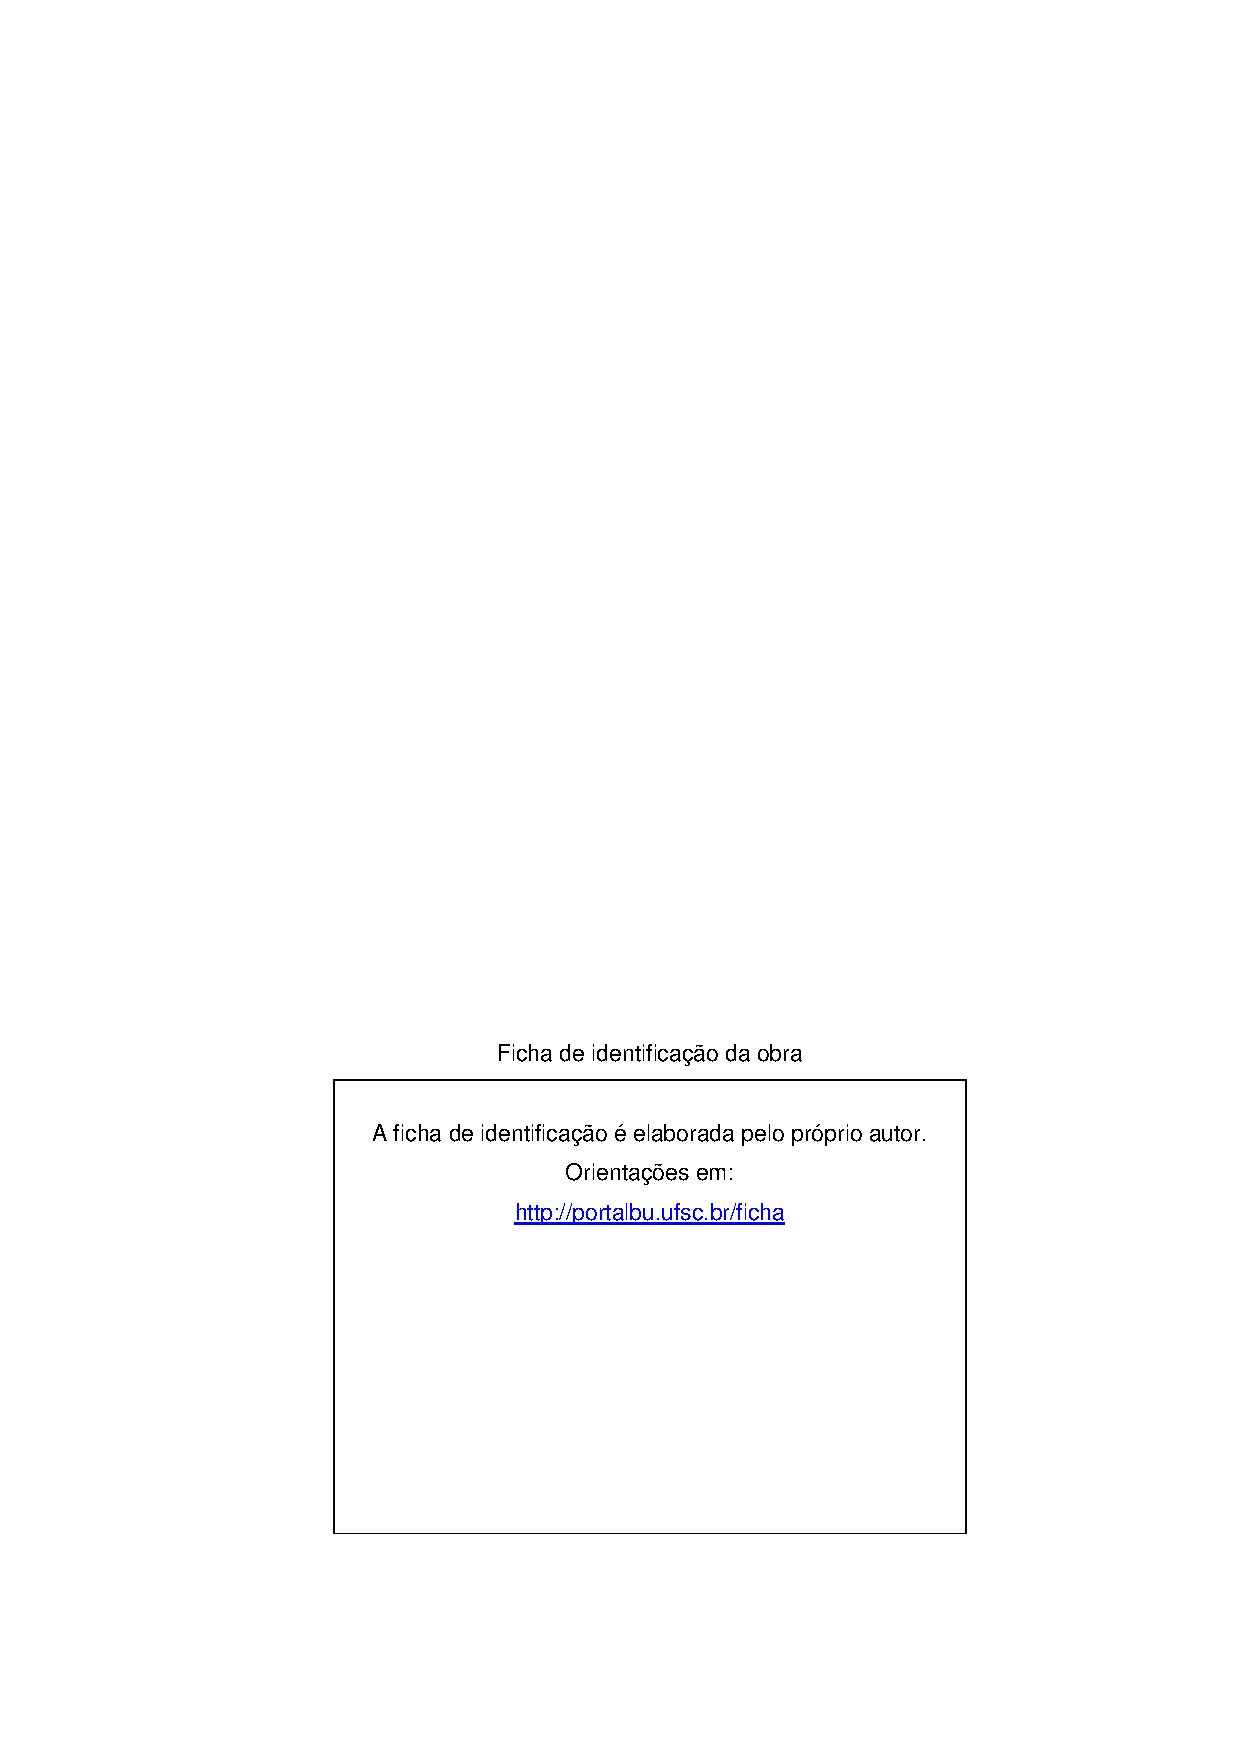
\includepdf{beforetext/Ficha_Catalografica.pdf}
\end{fichacatalografica}
% ---

% ---
% Inserir folha de aprovação
% ---
\begin{folhadeaprovacao}
	\OnehalfSpacing
	\centering
	\imprimirautor\\%
	\vspace*{10pt}		
	\textbf{\imprimirtitulo}%
	\ifnotempty{\imprimirsubtitulo}{:~\imprimirsubtitulo}\\%
	%		\vspace*{31.5pt}%3\baselineskip
	\vspace*{\baselineskip}
	%\begin{minipage}{\textwidth}
	% ~do~\imprimirprograma~do~\imprimircentro~da~\imprimirinstituicao~para~a~obtenção~do~título~de~\imprimirformacao.
	Esta~\imprimirtipotrabalho~foi julgada adequado para obtenção do Título de “\imprimirformacao” e aprovada em sua forma final pelo~\imprimirprograma. \\
		\vspace*{\baselineskip}
	\imprimirlocal, \imprimirdata. \\
	\vspace*{2\baselineskip}
	\assinatura{\OnehalfSpacing\imprimircoordenador \\ \imprimircoordenadorRotulo~do Curso}
	\vspace*{2\baselineskip}
	\textbf{Banca Examinadora:} \\
	\vspace*{\baselineskip}
	\assinatura{\OnehalfSpacing\imprimirorientador \\ \imprimirorientadorRotulo}
	%\end{minipage}%
	\vspace*{\baselineskip}
	\assinatura{Prof. Pedro Luiz Borges Chaffe, Dr.\\
	Avaliador \\
	Universidade Federal de Santa Catarina}

	\vspace*{\baselineskip}
	\assinatura{Profa. Taciana Toledo de Almeida Albuquerque, Dra.\\
	Avaliadora \\
	Universidade Federal de Minas Gerais}

	\vspace*{\baselineskip}
	\assinatura{Prof. Rizzieri Pedruzzi, Dr.\\
	Avaliador \\
	Universidade do Estado do Rio de Janeiro}

	\vspace*{\baselineskip}
	\assinatura{Prof. Alejandro Durán Carrillo de Albornoz, Dr.\\
	Avaliador \\
	Universidade de Havana, Cuba}

\end{folhadeaprovacao}
% ---

% ---
% Dedicatória
% ---
\begin{dedicatoria}
	\vspace*{\fill}
	\noindent
	\begin{adjustwidth*}{}{5.5cm}     
		À minha vó Olga, quem me ensinou a escrever.
	\end{adjustwidth*}
\end{dedicatoria}
% ---

% ---
% Agradecimentos
% ---
\begin{agradecimentos}
	Primeiramente agradeço a Deus por me conceder a inspiração, energia e o sustento para concluir este trabalho. Agradeço especialmente aos professores Henrique de Melo Lisboa, Alejandro Durán Carrillo de Albornoz e Alejandro García Ramírez que depositaram sua confiança em 2014 me concedendo a oportunidade que me conduziu até este estágio da minha carreira profissional, exatamente 10 anos depois. Minha profunda gratidão ao professor Leonardo Hoinaski que me ofereceu o desafio de assumir a empreitada deste projeto, juntamente com seu total apoio em todas as áreas, lutando lado a lado, suportando nos momentos difíceis e corrigindo nos momentos de vacilo. Meus agradecimentos vão também para o professor Davide Franco por me acolher e conduzir nos primeiros anos de doutorado. 

	Agradeço a minha esposa por suportar pacientemente os sacrifícios advindos de uma tese de doutorado, por perdoar minhas ausências e por encorajar nos momentos de desânimo. Aos meus sogros que me acolheram como um filho. À minha mãe por ser minha principal fã, por seus conselhos e seu sólido suporte. Ao meu caro irmão Andy Blanco por preparar o caminho para minha entrada no LCQAr e por seu apoio incondicional nos primeiros anos. Aos amigos que ganhei e que anseiam minha volta à vida social. Aos meus colegas de laboratório Camilo, Robson, Thiago e Otávio pela parceria e a amizade na ciência brasileira, a Gabriel Ratão e a Jean, que foram verdadeiros companheiros de luta e fizeram possível que este trabalho acontecesse. Ao PPGEA da UFSC que me abriu suas portas ao programa num momento de grandes incertezas e instabilidades.

	Agradeço à empresa Dynamox e seu CEO Guillaume Barrault por me oferecer emprego quando a bolsa de doutorado não foi suficiente para o sustento, e por me possibilitar concluir a pesquisa concedendo todo o suporte e flexibilidade possíveis. Ao coordenador João Pedro dos Reis que tem se tornado um amigo e uma importante fonte de encorajamento. Por todo o conhecimento adquirido através dos meus colegas que possibilitou refinar muitas etapas da pesquisa, em especial ao próprio João e ao Daniel Schröder. Ao Marcos Barp por oferecer seu tempo e conhecimento para resolver "pepinos" de séries temporais.

	À Mãe gentil brasileira, que em berço esplêndido me acolheu, enquanto Saturno devorava os seus filhos.
\end{agradecimentos}
% ---

% ---
% Epígrafe
% ---
\begin{epigrafe}
	\vspace*{\fill}
	\begin{flushright}
		\textit{``Ó Senhor, que variedade há nas tuas obras! Fizeste todas com sabedoria; a terra está cheia das tuas riquezas.
		Também o vasto mar, onde se movem seres inumeráveis, animais pequenos e grandes.
		Ali passam os navios, e o Leviatã que formaste para nele se recrear.
		Todos esperam de ti que lhes dês o sustento a seu tempo.''\\
			(Salmo de Davi)}
	\end{flushright}
\end{epigrafe}
% ---

% ---
% RESUMOS
% ---

% resumo em português
\setlength{\absparsep}{18pt} % ajusta o espaçamento dos parágrafos do resumo
\begin{resumo}
	\SingleSpacing
	O monitoramento da qualidade do ar tem experimentado uma mudança de paradigma com a incorporação de sensores de baixo custo. Estes equipamentos têm potencial para aumentar a resolução espaço-temporal dos dados de poluentes, assim como diversificar e simplificar as aplicações de monitoramento. Todavia, o volume e a diversidade de aplicações com este tipo de sensores encontra-se restrito pela baixa portabilidade de uma aplicação para outra e pela concentração de iniciativas maioritariamente em países desenvolvidos. Neste trabalho foi desenvolvido um sistema para o monitoramento de baixo custo da qualidade do ar: a iniciativa CLEAN (Collaborative Low-cost Environmental Air quality Network). O sistema foi desenvolvido com uma arquitetura modular possibilitando o reaproveitamento de funcionalidades comuns entre aplicações, direcionando assim os esforços de desenvolvimento à implementação dos requisitos específicos de cada aplicação particular. CLEAN engloba um conjunto de subsistemas que incluem: uma \textit{API} para registro e acesso a dados de monitores de baixo custo, bibliotecas de \textit{firmware} e elementos de \textit{hardware} para o desenvolvimento de monitores de baixo custo. No trabalho também foram desenvolvidos monitores de baixo custo para comporem a rede CLEAN. Um deles foi instalado junto a uma estação de monitoramento de referência da qualidade do ar, para validação e correção das suas leituras por um período de 5 meses. No trabalho propõe-se uma metodologia de correção das leituras do equipamento, a partir das medições coletadas pela estação de referência. Para isso foram ajustados modelos de regressão baseados em redes neurais Perceptron Multicamadas, Florestas Aleatórias, K Vizinhos mais Próximos e regressão Linear Multivariada. Os modelos, diferentemente de outros trabalhos que realizam correções das leituras de sensores de baixo custo, consideraram, como variáveis de entrada, as leituras de diferentes modelos de sensores para obter as medidas de um determinado gás. No caso em questão, foram utilizados sensores de baixo custo do fabricante Alphasense, sensíveis aos gases Monóxido de Carbono (\textit{CO}), Dióxido de Nitrogênio (\textit{NO2}), Ozônio (\textit{O3}) e Material Particulado (\textit{MP10}). A metodologia de correção desenvolvida, considera o conjunto das leituras de todos os sensores e da temperatura para obter as medições de um único gás. Com essa metodologia obtiveram-se modelos de correção com valores de R2 de até 0.6 para a medição de \textit{O3} utilizando uma rede neural Perceptron Multicamadas. Os modelos obtidos para correção das medidas de \textit{MP10}, \textit{NO2} e \textit{CO}, se comparados com as correções que consideravam um único modelo de sensor, apresentaram um incremento no valor de R2 de \textit{R2 < 0} até 0.18, 0.14 e 0.07 respectivamente.A metodologia proposta nesta pesquisa mostrou-se robusta para trabalhar com dados de baixa qualidade e acrescentar valor a leituras ruidosas e com falhas nos sensores. O trabalho traz como principais contribuições um marco de trabalho colaborativo para o desenvolvimento e interconexão de sensores de baixo custo, assim como uma metodologia para calibração dos sensores com dados muito ruidosos, em uma aplicação real e em ambiente não controlado.
	
	\textbf{Palavras-chave}: Monitoramento da qualidade do ar, rede colaborativa, sensores de gases de baixo custo, sistemas embarcados, \acrshort{api}, modelos de regressão, aprendizado de máquinas
\end{resumo}

% resumo em inglês
\begin{resumo}[Abstract]
	\SingleSpacing
	\begin{otherlanguage*}{english}
		Air quality monitoring has experienced a paradigm shift with the incorporation of low-cost sensors. This equipment has the potential to increase the spatio-temporal resolution of pollutant data, as well as diversify and simplify monitoring applications. However, the volume and diversity of applications with this type of sensor are restricted by the low portability of one application to another and the concentration of initiatives mainly in developed countries. In this work, a system was developed for low-cost monitoring of air quality: the CLEAN (Collaborative Low-cost Environmental Air Quality Network) initiative. The system was developed with a modular architecture enabling the reuse of common functionalities between applications, thus directing development efforts to implement the specific requirements of each particular application. CLEAN encompasses a set of subsystems that include: an API for recording and accessing data from low-cost monitors, firmware libraries, and hardware elements for developing low-cost monitors. In the work, low-cost monitors were also developed to form part of the CLEAN network. One of them was installed next to an air quality reference monitoring station, to validate and correct its readings for a period of 5 months. The work proposes a methodology for correcting equipment readings, based on measurements collected by the reference station. For this, regression models based on Multilayer Perceptron neural networks, Random Forests, K Nearest Neighbors, and Multivariate Linear regression were adjusted. The models, unlike other works that perform corrections to readings from low-cost sensors, considered, as input variables, the readings from different sensor models to obtain measurements of a given gas. In the case in question, low-cost sensors from the manufacturer Alphasense were used, sensitive to the gases Carbon Monoxide (CO), Nitrogen Dioxide (NO2), Ozone (O3), and Particulate Matter (PM10). The correction methodology developed considers the set of readings from all sensors and temperature to obtain measurements of a single gas. With this methodology, correction models with R2 values of up to 0.6 were obtained for measuring O3 using a Multilayer Perceptron neural network. The models obtained to correct the measurements of PM10, NO2, and CO, when compared with the corrections that considered a single sensor model, showed an increase in the R2 value from R2 < 0 to 0.18, 0.14, and 0.07 respectively. The methodology proposed in this research proved to be robust in working with low-quality data and adding value to noisy readings and sensor failures. The main contributions of the work are a collaborative work framework for the development and interconnection of low-cost sensors, as well as a methodology for calibrating sensors with very noisy data, in a real application and an uncontrolled environment.

		\textbf{Keywords}: Air quality monitoring, collaborative network, low-cost gas sensors, embedded systems, \acrshort{api}, regression models, machine learning
	\end{otherlanguage*}
\end{resumo}

{%hidelinks
	\hypersetup{hidelinks}
	% ---
	% inserir lista de ilustrações
	% ---
	\pdfbookmark[0]{\listfigurename}{lof}
	\listoffigures*
	\cleardoublepage
	% ---
	
	% ---
	% inserir lista de tabelas
	% ---
	\pdfbookmark[0]{\listtablename}{lot}
	\listoftables*
	\cleardoublepage
	% ---
	
	% ---
	% inserir lista de abreviaturas e siglas (devem ser declarados no preambulo)
	% ---
	% \imprimirlistadesiglas
	% ---
	
	% ---
	% inserir lista de símbolos (devem ser declarados no preambulo)
	% ---
	% \imprimirlistadesimbolos
	% ---
	\pdfbookmark[0]{Lista de siglas}{los}
	\printnoidxglossary[type=acronym, sort=use, title=Lista de siglas, toctitle=Lista de siglas]
	\cleardoublepage

	% ---
	% inserir o sumario
	% ---
	\pdfbookmark[0]{\contentsname}{toc}
	\tableofcontents*
	\cleardoublepage
	
}%hidelinks
% ---